\documentclass{standalone}
\usepackage{tikz}
\begin{document}
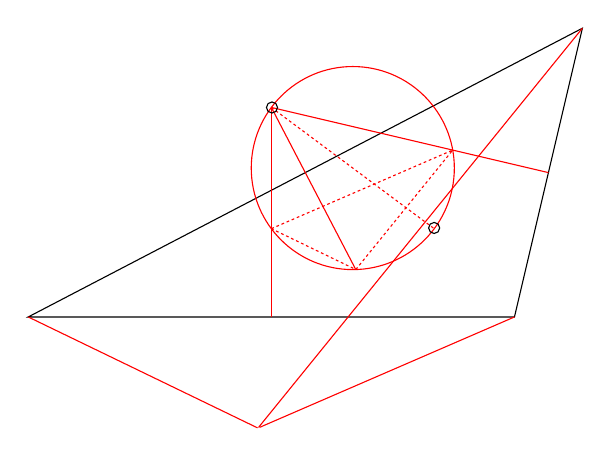
\begin{tikzpicture}[x=1pt,y=1pt]
\draw (241.93,-101.13) -- (41.69,-205.46) -- (217.39,-205.46) -- cycle;
\draw[red] (158.97,-151.66) circle (36.69);
\draw[red, dash pattern=on 1pt] (129.54,-129.75) -- (188.40,-173.57);
\draw[red] (129.54,-129.75) -- (129.54,-205.47);
\draw[red] (129.54,-129.75) -- (229.66,-153.30);
\draw[red] (129.54,-129.75) -- (160.05,-188.33);
\draw[red] (41.69,-205.46) -- (124.55,-245.54);
\draw[red] (241.93,-101.13) -- (124.91,-245.37);
\draw[red] (217.39,-205.46) -- (125.31,-245.35);
\draw (129.77,-129.77) circle (2.00);
\draw (188.37,-173.30) circle (2.00);
\draw[red, dash pattern=on 1pt] (129.54,-173.56) -- (195.08,-145.16) -- (160.06,-188.32) -- cycle;
\end{tikzpicture}
\end{document}
